% !TeX spellcheck = en_GB 
\section{Validation}
Tensile tests were performed on an Instron 3366 Universal Testing machine at \SI{5}{\milli\meter\per\minute}.
Prints were manufactured on an Ultimaker S5 in 5-fold with Ultimaker Green Tough PLA and Ultimaker PP using the default \SI{0.1}{\milli\meter} layer thickness profile,
with \SI{100}{\percent} infill and a custom brim to make sure both materials stick to the build plate.
For PP we print the outer before the inner walls so as to improve the dimensional accuracy. % on TPLA we forgot to edit those settings
In order to deal with the various widths of the beams we generate toolpaths using the Cura Arachne Engine beta release\cite{CuraArachne},
which implements the framework for generating variable line width toolpaths from \cite{Kuipers2020}.
The Inward Distributed and the Distributed strategy were used on TPLA and PP respectively.
See \cref{fig:gcode}.



\begin{figure}
	\setlength{\figheight}{.13\columnwidth}
	\centering
	\begin{subfigure}[B]{.2\columnwidth}
		\centering
		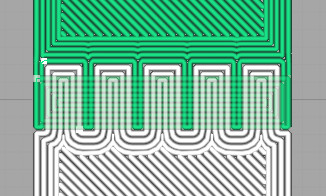
\includegraphics[height=\figheight]{sources/testing/straight_gcode.jpg}
		\caption{Straight}
		\label{fig:gcode_straight}
	\end{subfigure}
	\begin{subfigure}[B]{.2\columnwidth}
		\centering
		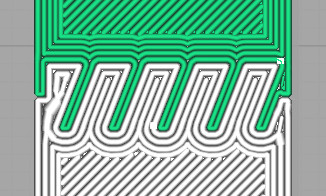
\includegraphics[height=\figheight]{sources/testing/diagonal_gcode.jpg}
		\caption{Diagonal}
		\label{fig:gcode_diagonal}
	\end{subfigure}
	\begin{subfigure}[B]{.24\columnwidth}
		\centering
		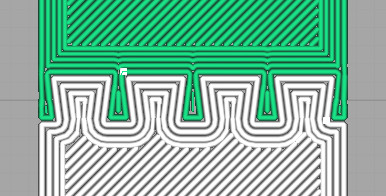
\includegraphics[height=\figheight]{sources/testing/suture_gcode.jpg}
		\caption{Trap. suture}
		\label{fig:gcode_suture}
	\end{subfigure}
	\begin{subfigure}[B]{.24\columnwidth}
		\centering
		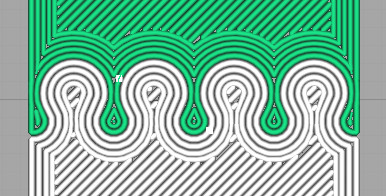
\includegraphics[height=\figheight]{sources/testing/jigsaw_gcode.jpg}
		\caption{Jigsaw}
		\label{fig:gcode_jigsaw}
	\end{subfigure}
	\caption{Example of gcodes generated with Cura Arachne engine beta.}
	\label{fig:gcode}
\end{figure}



\begin{figure*}
	\centering
	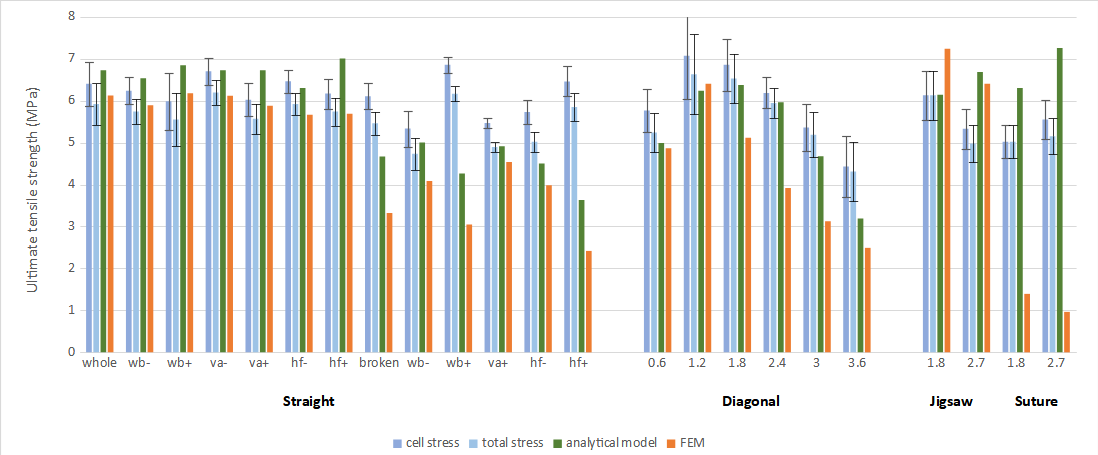
\includegraphics[width=\textwidth]{sources/testing/results.png}
	\caption{Test results compared to the predictions according to the analytical model and the RBF network fitted to the simulation results. The straight model samples are labelled relative to the whole and broken optimum, while the rest is labelled by their $\wb$ value.}
	\label{fig:test_results}
\end{figure*}




\subsection{Model parameters}
\subsubsection{Straight}
The straight design suffers from the curse of dimensionality;
Even when setting $\wa=\SI{0.6}{\milli\meter}$, $\hc=\SI{0.1}{\milli\meter}$ and $L=\SI{3.6}{\milli\meter}$,
there are still the three free design variables $\wb$, $\va$ and $\hf$ to determine.
With 5 specimens per sample point and limited resources, the total number of data points we are able to test is limited.
We therefore chose to sample close to the two optima of the analytical models: whole and broken, as well as deviations from those optima in each of the directions along a design variable.
See \cref{fig:test_points_straight}.

Each specimen has $5\times5$ cells.
Because the repetition of cells is broken at the sides of the specimen, the boundary cells are adjusted for manufacturability and stability.
The specimens end with a TPLA finger on both sides and in crossbeams on both top and bottom.
See \cref{fig:test_straight_boundary_cells}.

\begin{figure}
	\centering
	\begin{subfigure}[B]{.24\columnwidth}
		\centering
		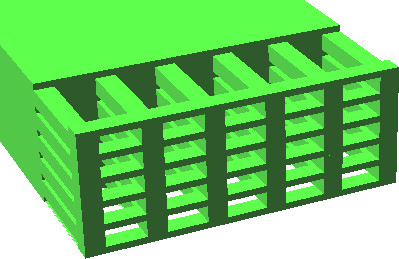
\includegraphics[width=\columnwidth]{sources/testing/straight_sample.jpg}
		\caption{Example print mesh near optimum}
		\label{fig:test_straight_boundary_cells}
	\end{subfigure}
	\begin{subfigure}[B]{.24\columnwidth}
		\centering
		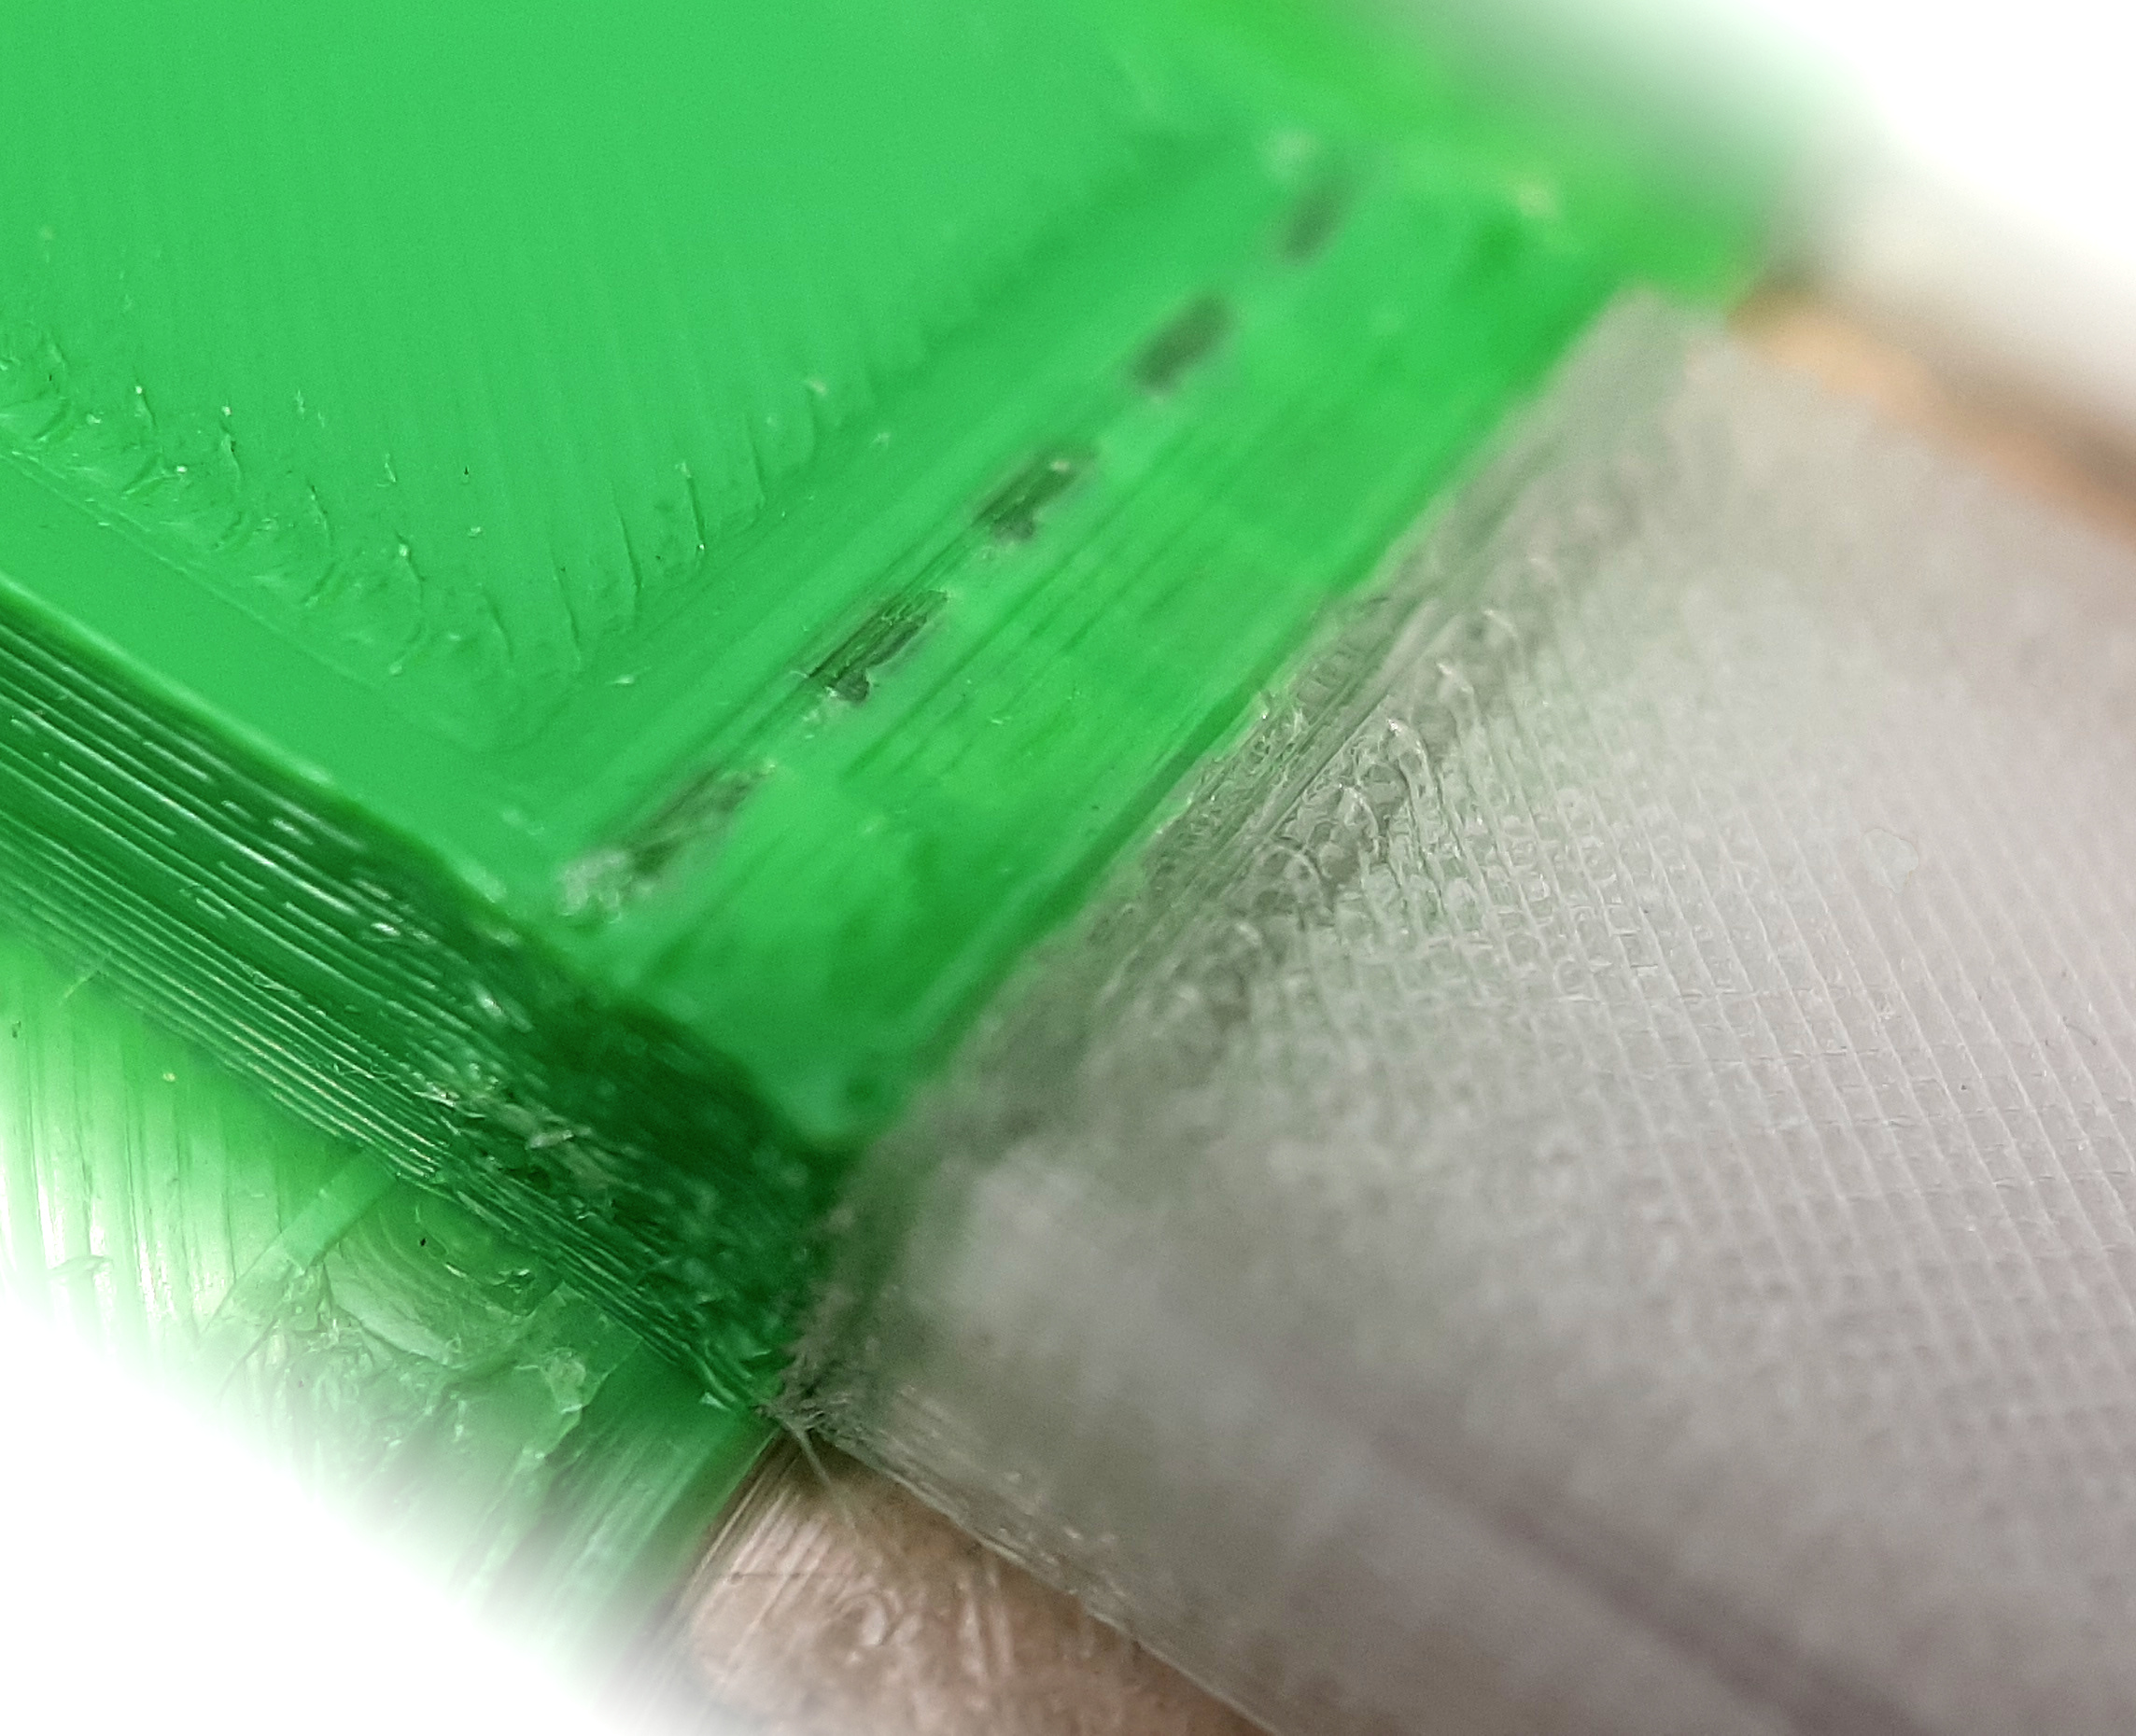
\includegraphics[width=\columnwidth]{sources/testing/straight_print.jpg}
		\caption{Example print near broken optimum}
	\end{subfigure}
	\begin{subfigure}[B]{.5\columnwidth}
		\centering
		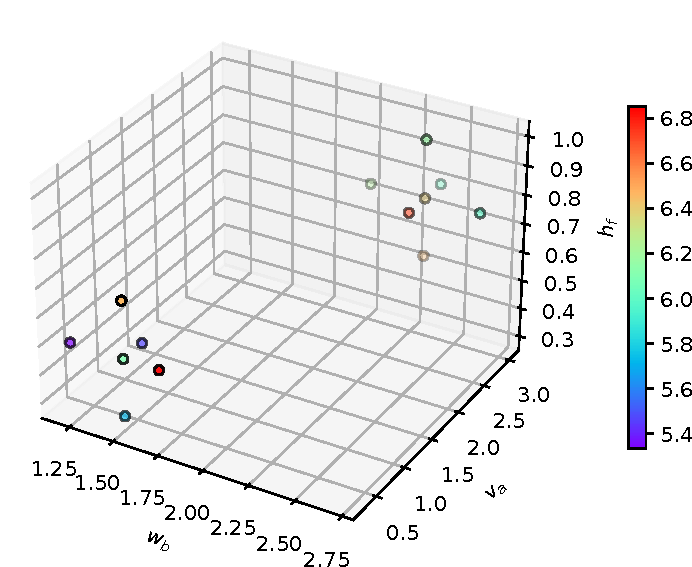
\includegraphics[width=\columnwidth]{sources/testing/straight_sample_points.pdf}
		\caption{Sampled points}
		\label{fig:test_points_straight}
	\end{subfigure}
	\caption{Experimental setup of straight design.}
\end{figure}





\subsubsection{Diagonal}
Because with a given $L=\SI{3.6}{\milli\meter}$, $h=\SI{0.2}{\milli\meter}$ and $\wa=\SI{0.6}{\milli\meter}$ the remaining design space is only one-dimensional,
we can simply sample various points along $\wb$: $(0.6, 1.2, 1.8, 2.4, 3.0, 3.6)$.
Each specimen contains 5 cells in the horizontal direction, but 13 repetition in Z.
Extra finger beams are added to the sides of the specimen to prevent any part of the beam to be less than $2\wmin=\SI{0.6}{\milli\meter}$ wide.
See \cref{fig:gcode_diagonal}.

\iffalse
\begin{figure}
	\centering
	\begin{subfigure}[B]{.24\columnwidth}
		\centering
		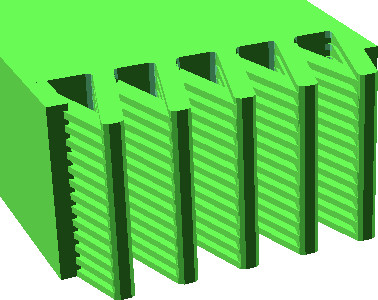
\includegraphics[width=\columnwidth]{sources/testing/diagonal_sample.jpg}
		\caption{Example print mesh}
		\label{fig:test_diagonal_boundary_cells}
	\end{subfigure}
	\begin{subfigure}[B]{.24\columnwidth}
		\centering
		\includegraphics[width=\columnwidth]{sources/testing/diagonal_print.jpg}
		\caption{Example print}
	\end{subfigure}
	\begin{subfigure}[B]{.5\columnwidth}
		\centering
		%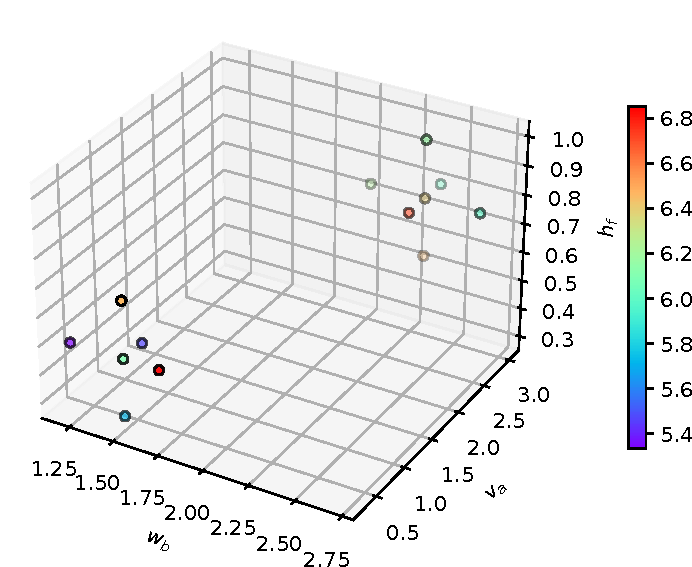
\includegraphics[width=\columnwidth]{sources/testing/straight_sample_points.pdf}
		\caption{Comparison of results to analytical model}
	\end{subfigure}
	\caption{Experimental setup of diagonal design.}
\end{figure}
\fi







\begin{figure}
	\centering
	\begin{subfigure}{.49\columnwidth}
		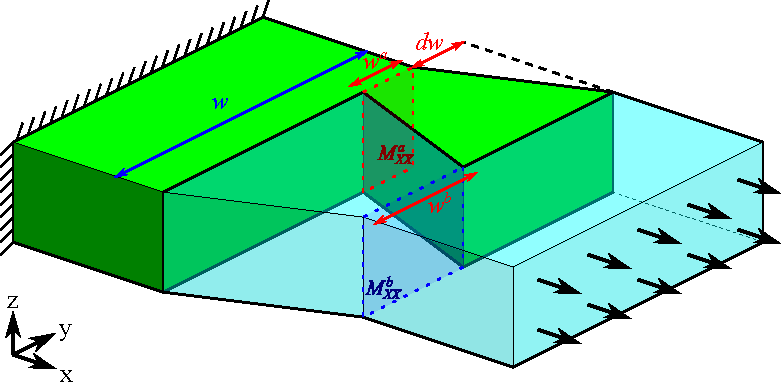
\includegraphics{sources/method/suture_model_v5.pdf}
		\caption{Trapezoidal suture}
		\label{fig:suture}
	\end{subfigure}
	\begin{subfigure}{.49\columnwidth}
		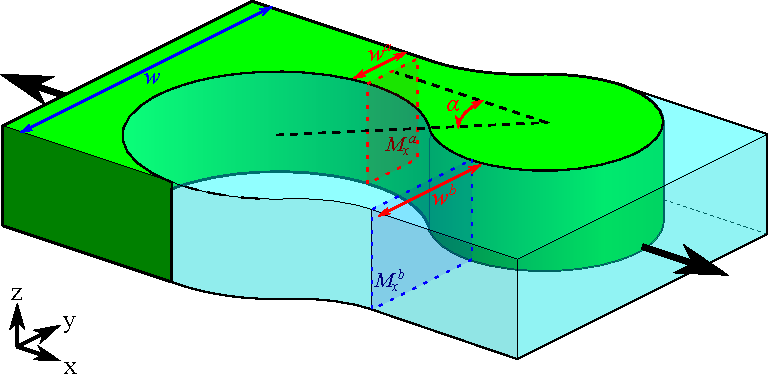
\includegraphics{sources/method/jigsaw_model_v5.pdf}
		\caption{Jigsaw}
		\label{fig:jigsaw}
	\end{subfigure}
	\caption{Simple 2D dovetail interlocking microstructures.}
	\label{fig:suture_jigsaw}
\end{figure}


\subsubsection{Dovetail interlocking}
We compared our interlocking structures against two interlocking designs: trapezoidal sutures and jigsaw interlocking.
See \cref{fig:suture_jigsaw}.
We used $\wa=2\wmin{a}$, $dw=\SI{0.3}{\milli\meter}$ and $L=2.4$ for the trapezoidal suture,
and $\wa=2\wmin{a}$ and $\alpha = \SI{35}{\degree}$ for the jigsaw interlocking design.
We printed samples with both $\wb=3\wa$ and $\wb=\nicefrac{\sigmafail{a}}{\sigmafail{b}}\wa = 4.48 \wa$.
%The latter value is optimized for tensile failure along $\myz{b}$. >> not true!!!
We used 6 and 4 repetition respectively and a height of \SI{5}{\milli\meter}.

Note that the jigsaw interlocking structure is quite similar to the trapezoidal suture, with the addition of semicircles to the ends of the trapezoids.
The total length $L$ of the jigsaw structure is \SI{2.96}{\milli\meter} and \SI{4.05}{\milli\meter} for the two $\wb$ values respectively,
so the $\lmax$ constraint is violated by that structure.

The boundaries of these two structures end in half a TPLA lobe, because that is the stiffer material.
In order to meet the minimum width constraint there, the sides of the specimen are extruded by $\wmin{a}$.



\subsection{Results}
After tensile testing we can observe various failure modes, such as in \cref{fig:failures}.
The tensile tests performed result in force-displacement graphs such as displayed in \cref{fig:force-displacement},
from which the ultimate tensile strength is derived.
Because the boundary cells deviate from the regular pattern, computing the ultimate tensile strength can be done in two ways, giving rise to two statistics.
We compute the \emph{cell stress} by dividing the maximum force of the force-displacement graphs by the number of cells and then divide it by the cross sectional area of the cell.
We compute the \emph{total stress} by dividing the force by the total cross-sectional area of the sample, including the extra geometry at the boundaries of the sample.
Ideally we would compensate for manufacturing inaccuracies by using measured dimensions of the specimens,
but measuring the internal geometry of the interlocking structure is practically infeasible, so we use the dimensions of the 3D mesh instead.


\begin{figure}
	\centering
	\begin{subfigure}[B]{.99\columnwidth}
		\centering
		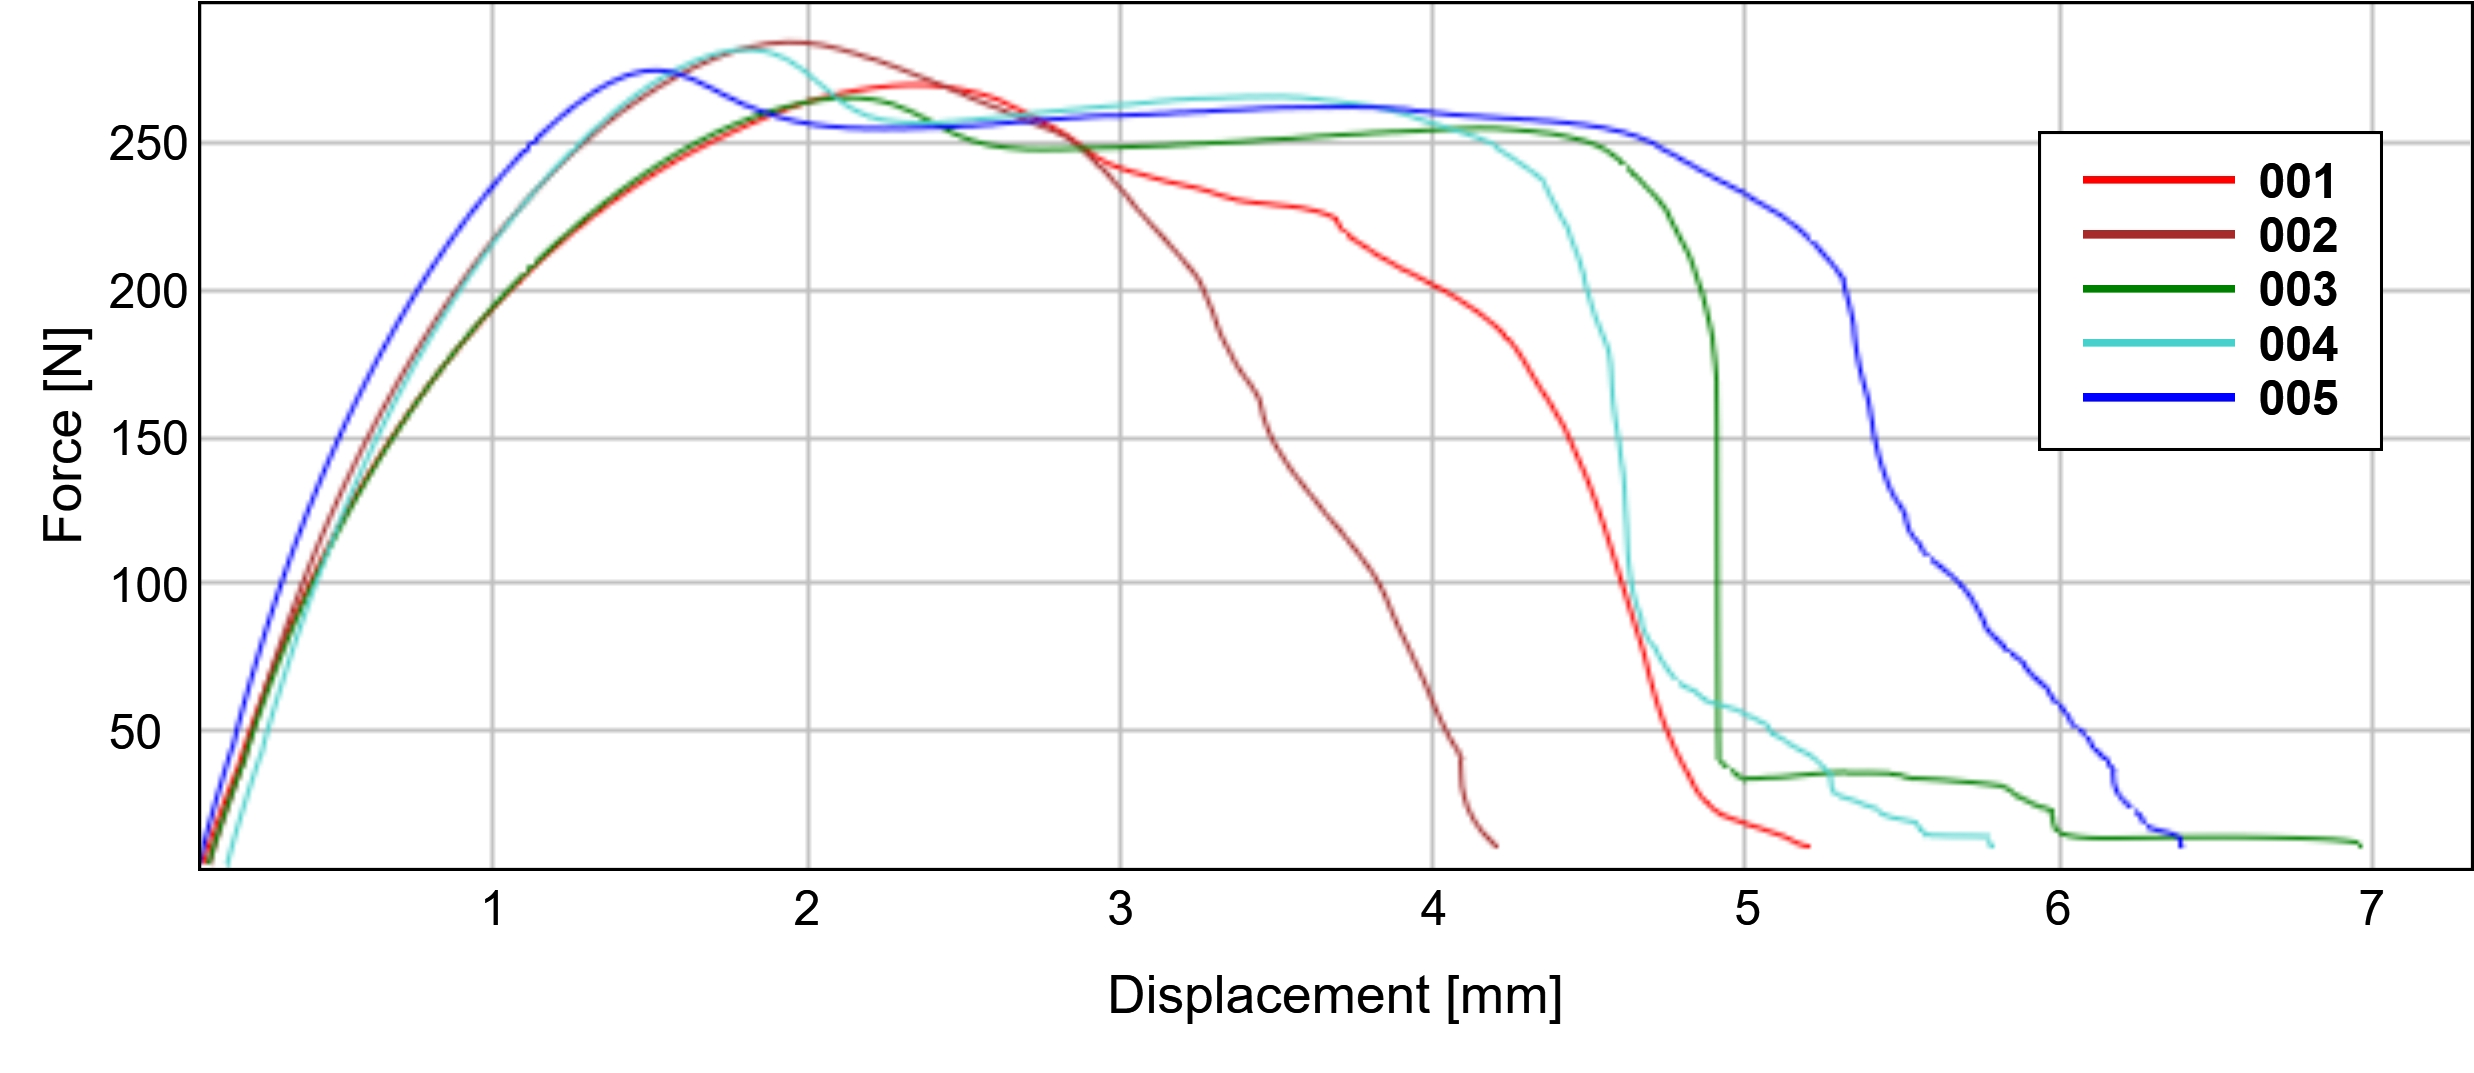
\includegraphics[width=\columnwidth]{sources/testing/force_displacement_J.png}
		\caption{Force-displacement graph.}
		\label{fig:force-displacement}
	\end{subfigure}
\setlength{\figwidth}{.19\columnwidth}
	\begin{subfigure}[B]{.99\columnwidth}
		\centering
		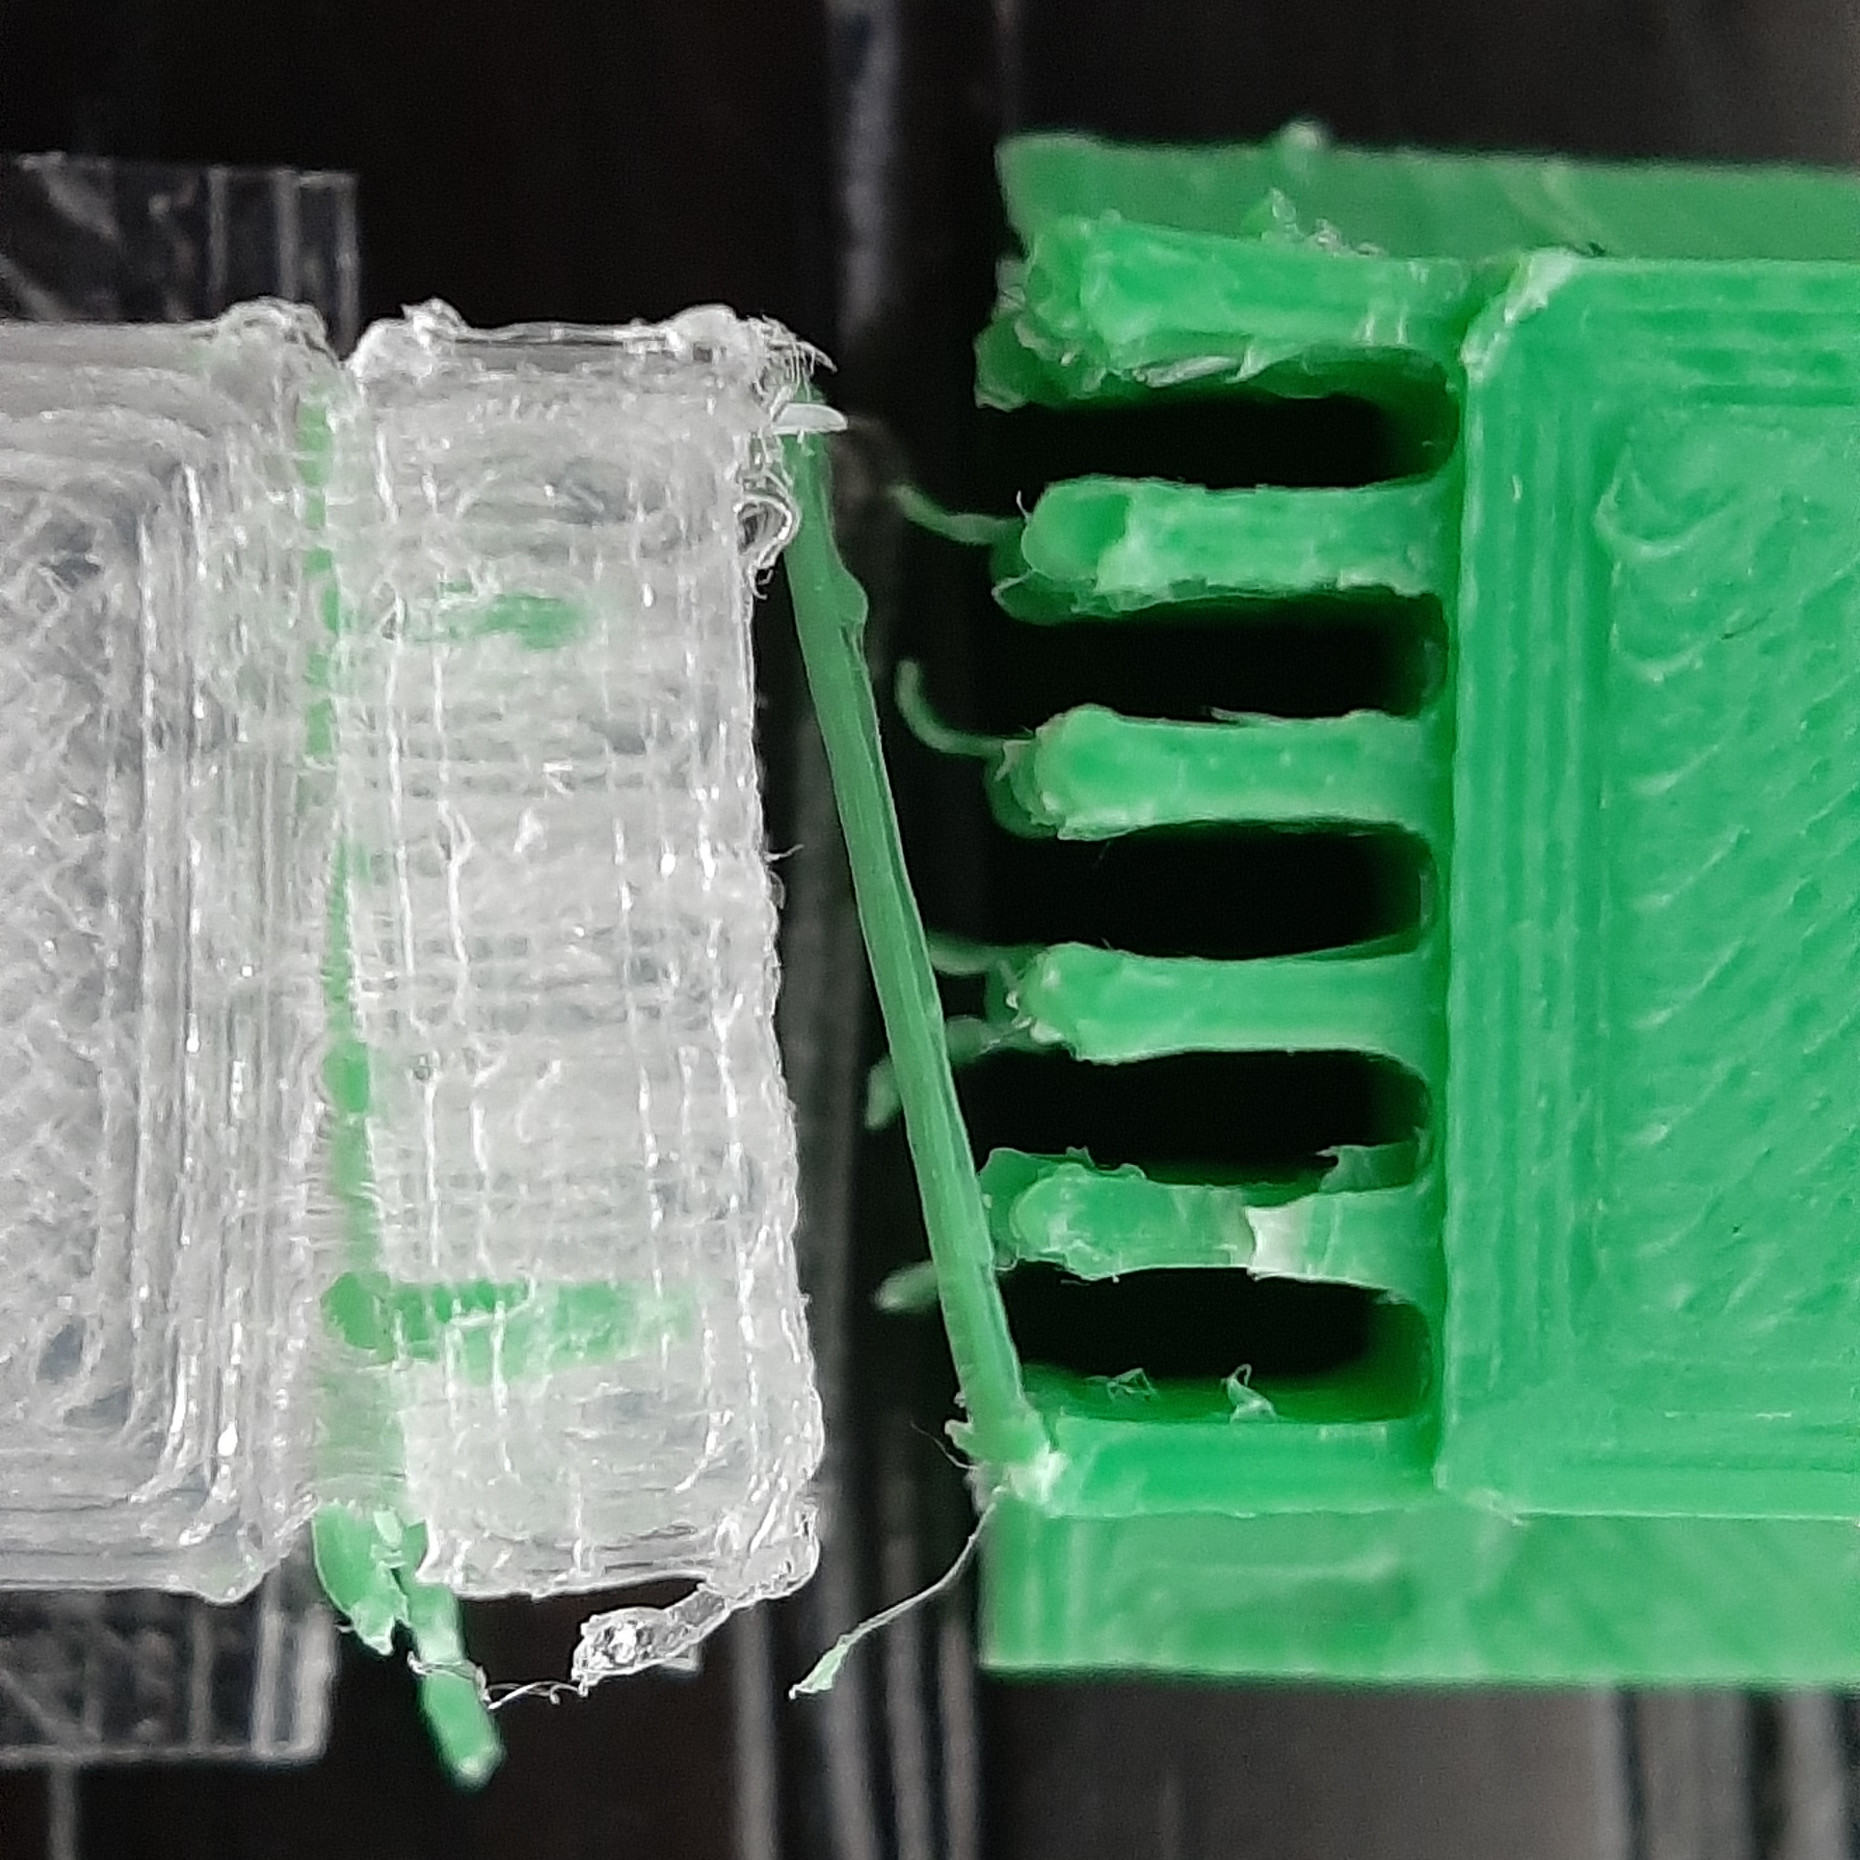
\includegraphics[width=\figwidth]{sources/testing/j1_cropped.jpg}
		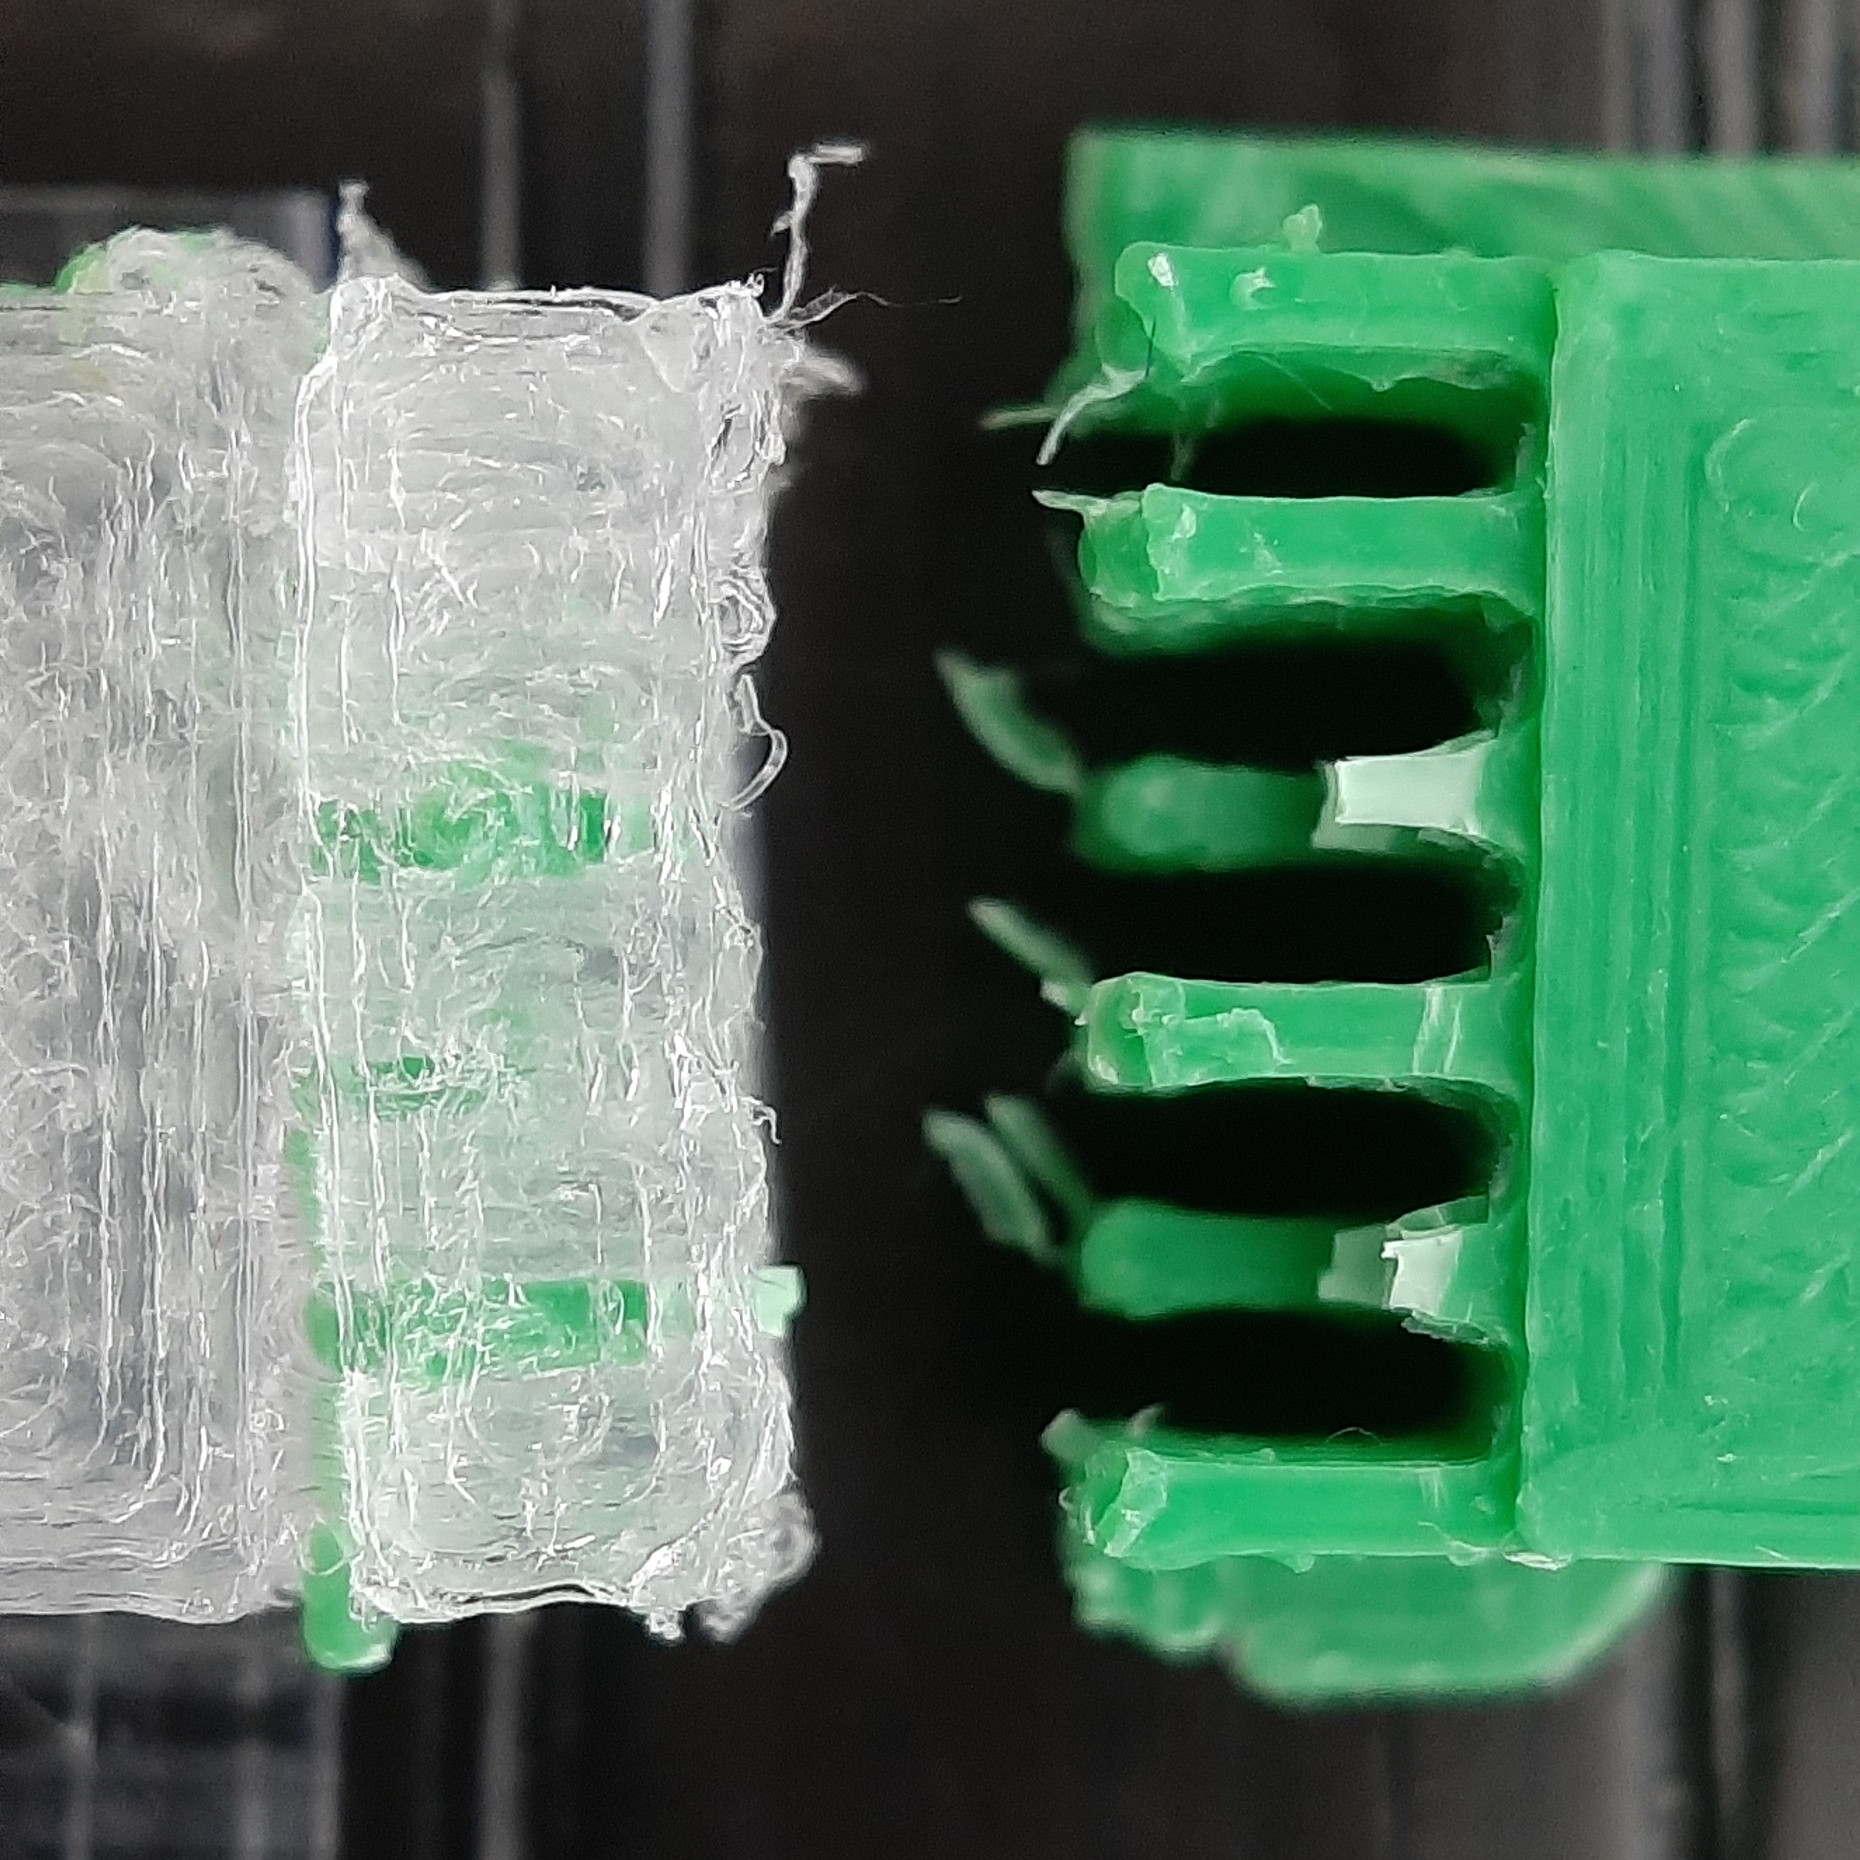
\includegraphics[width=\figwidth]{sources/testing/j2_cropped.jpg}
		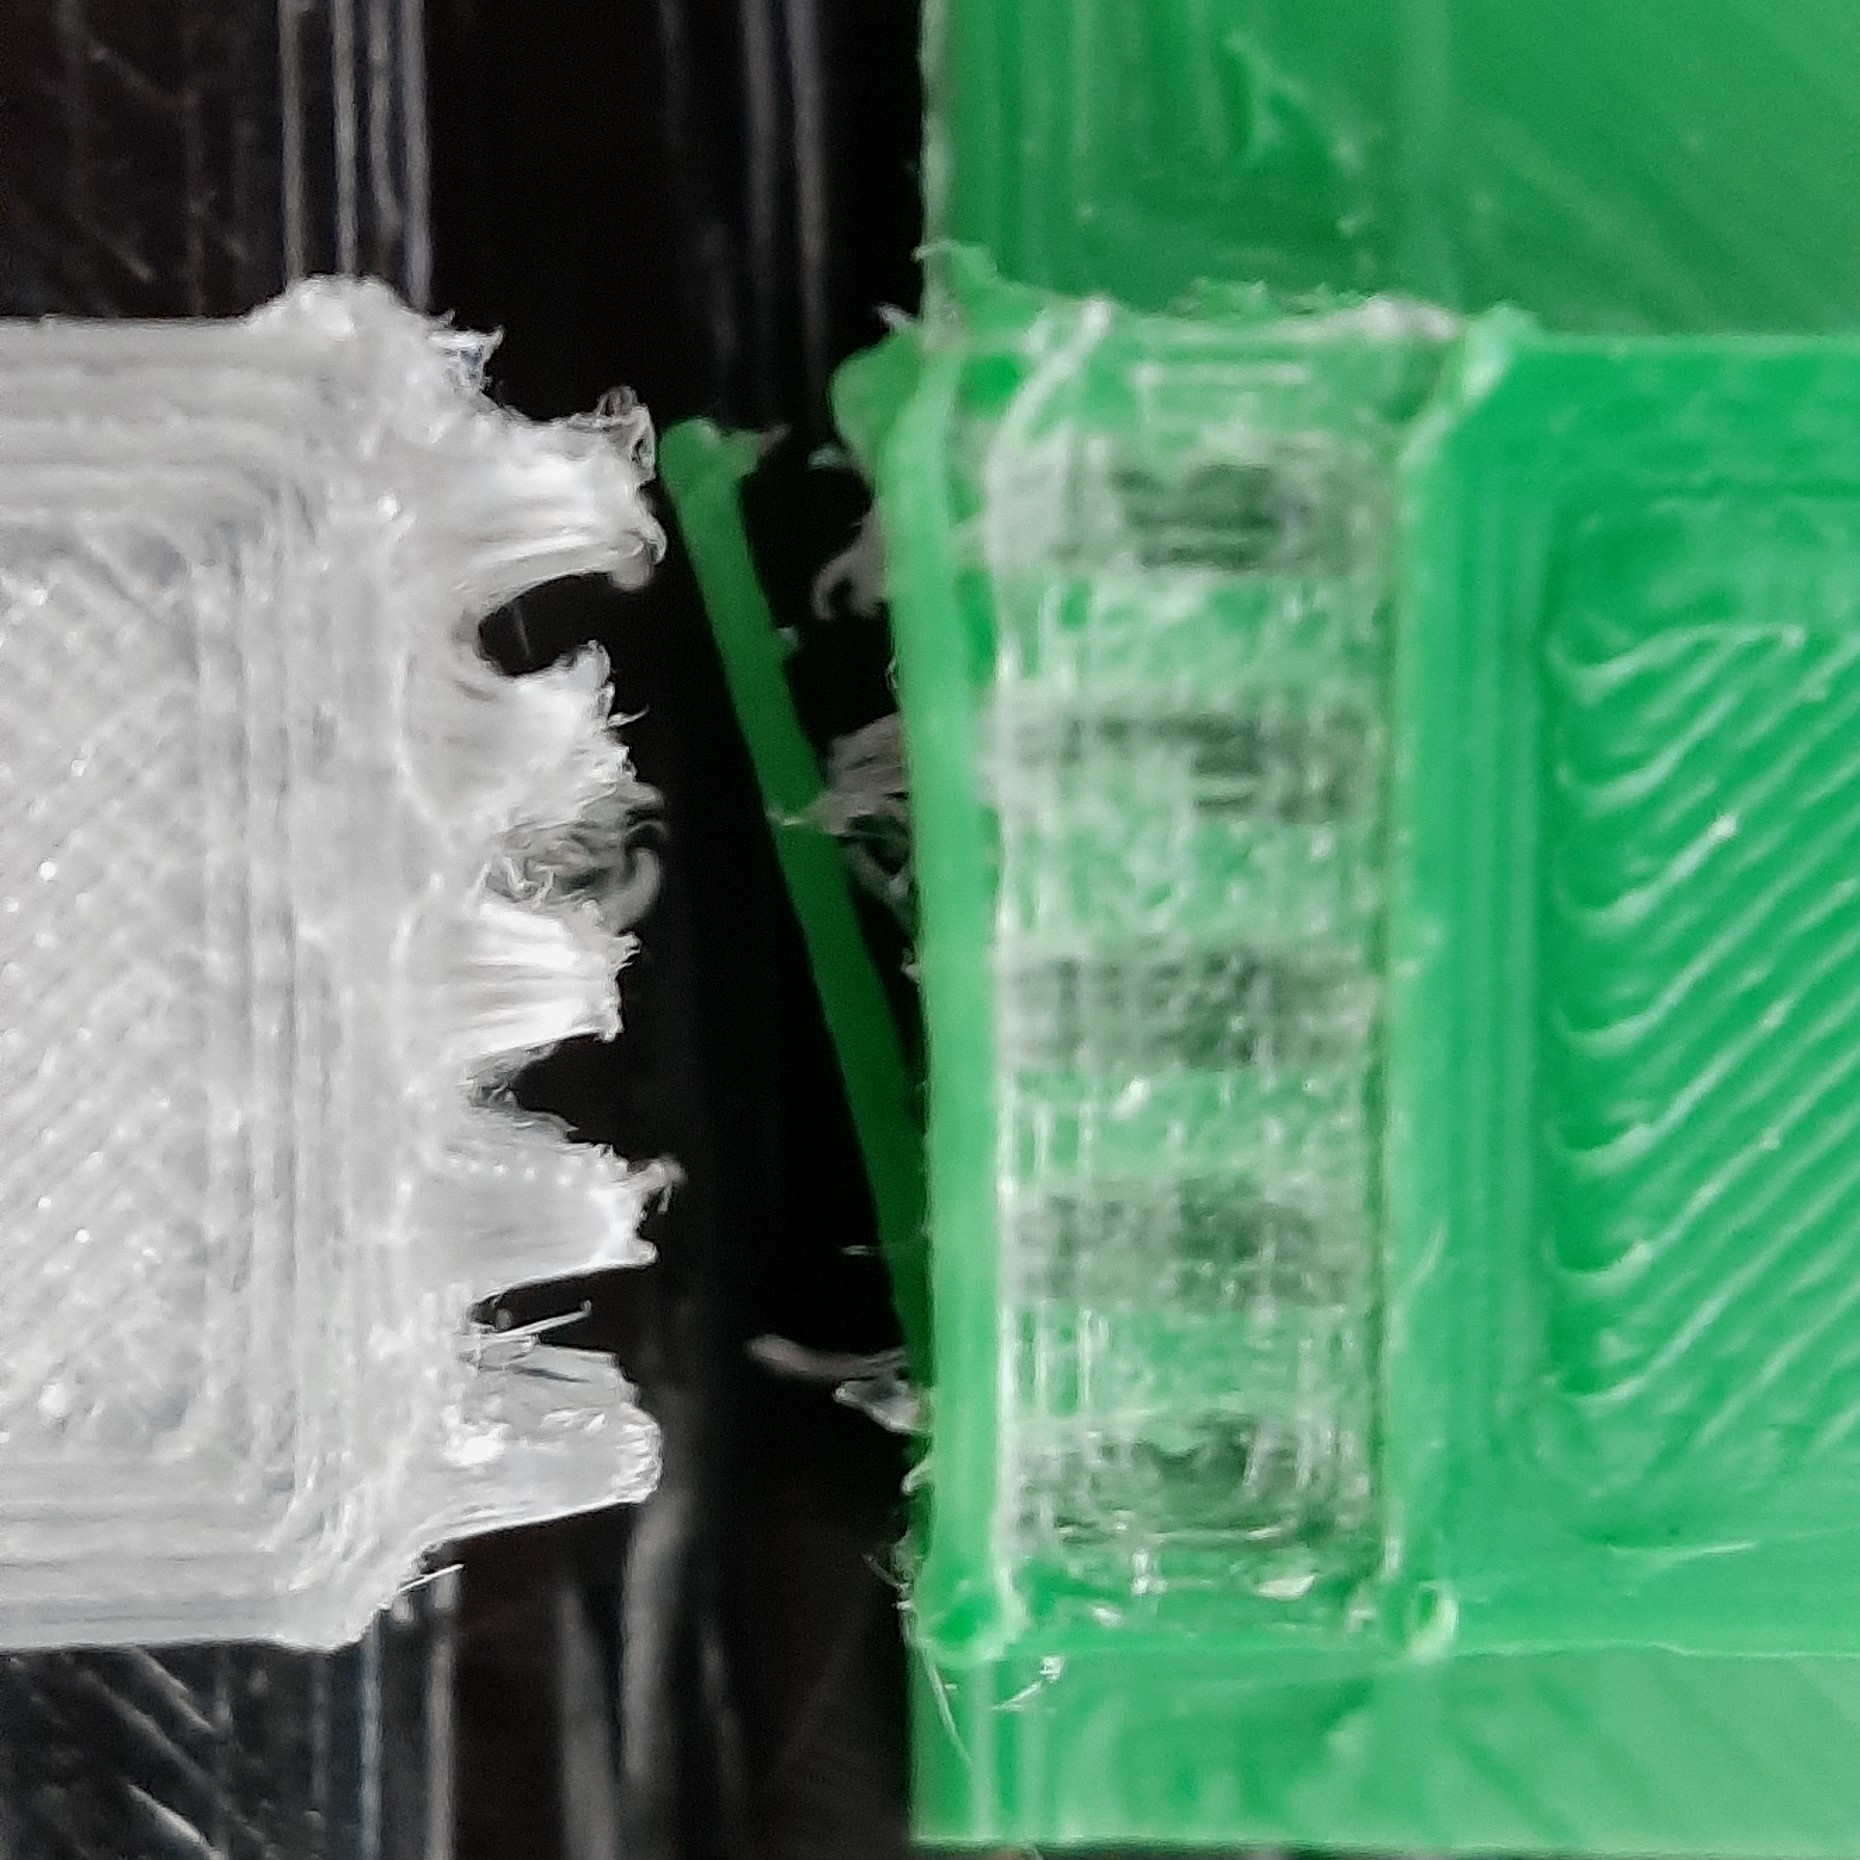
\includegraphics[width=\figwidth]{sources/testing/j3_cropped.jpg}
		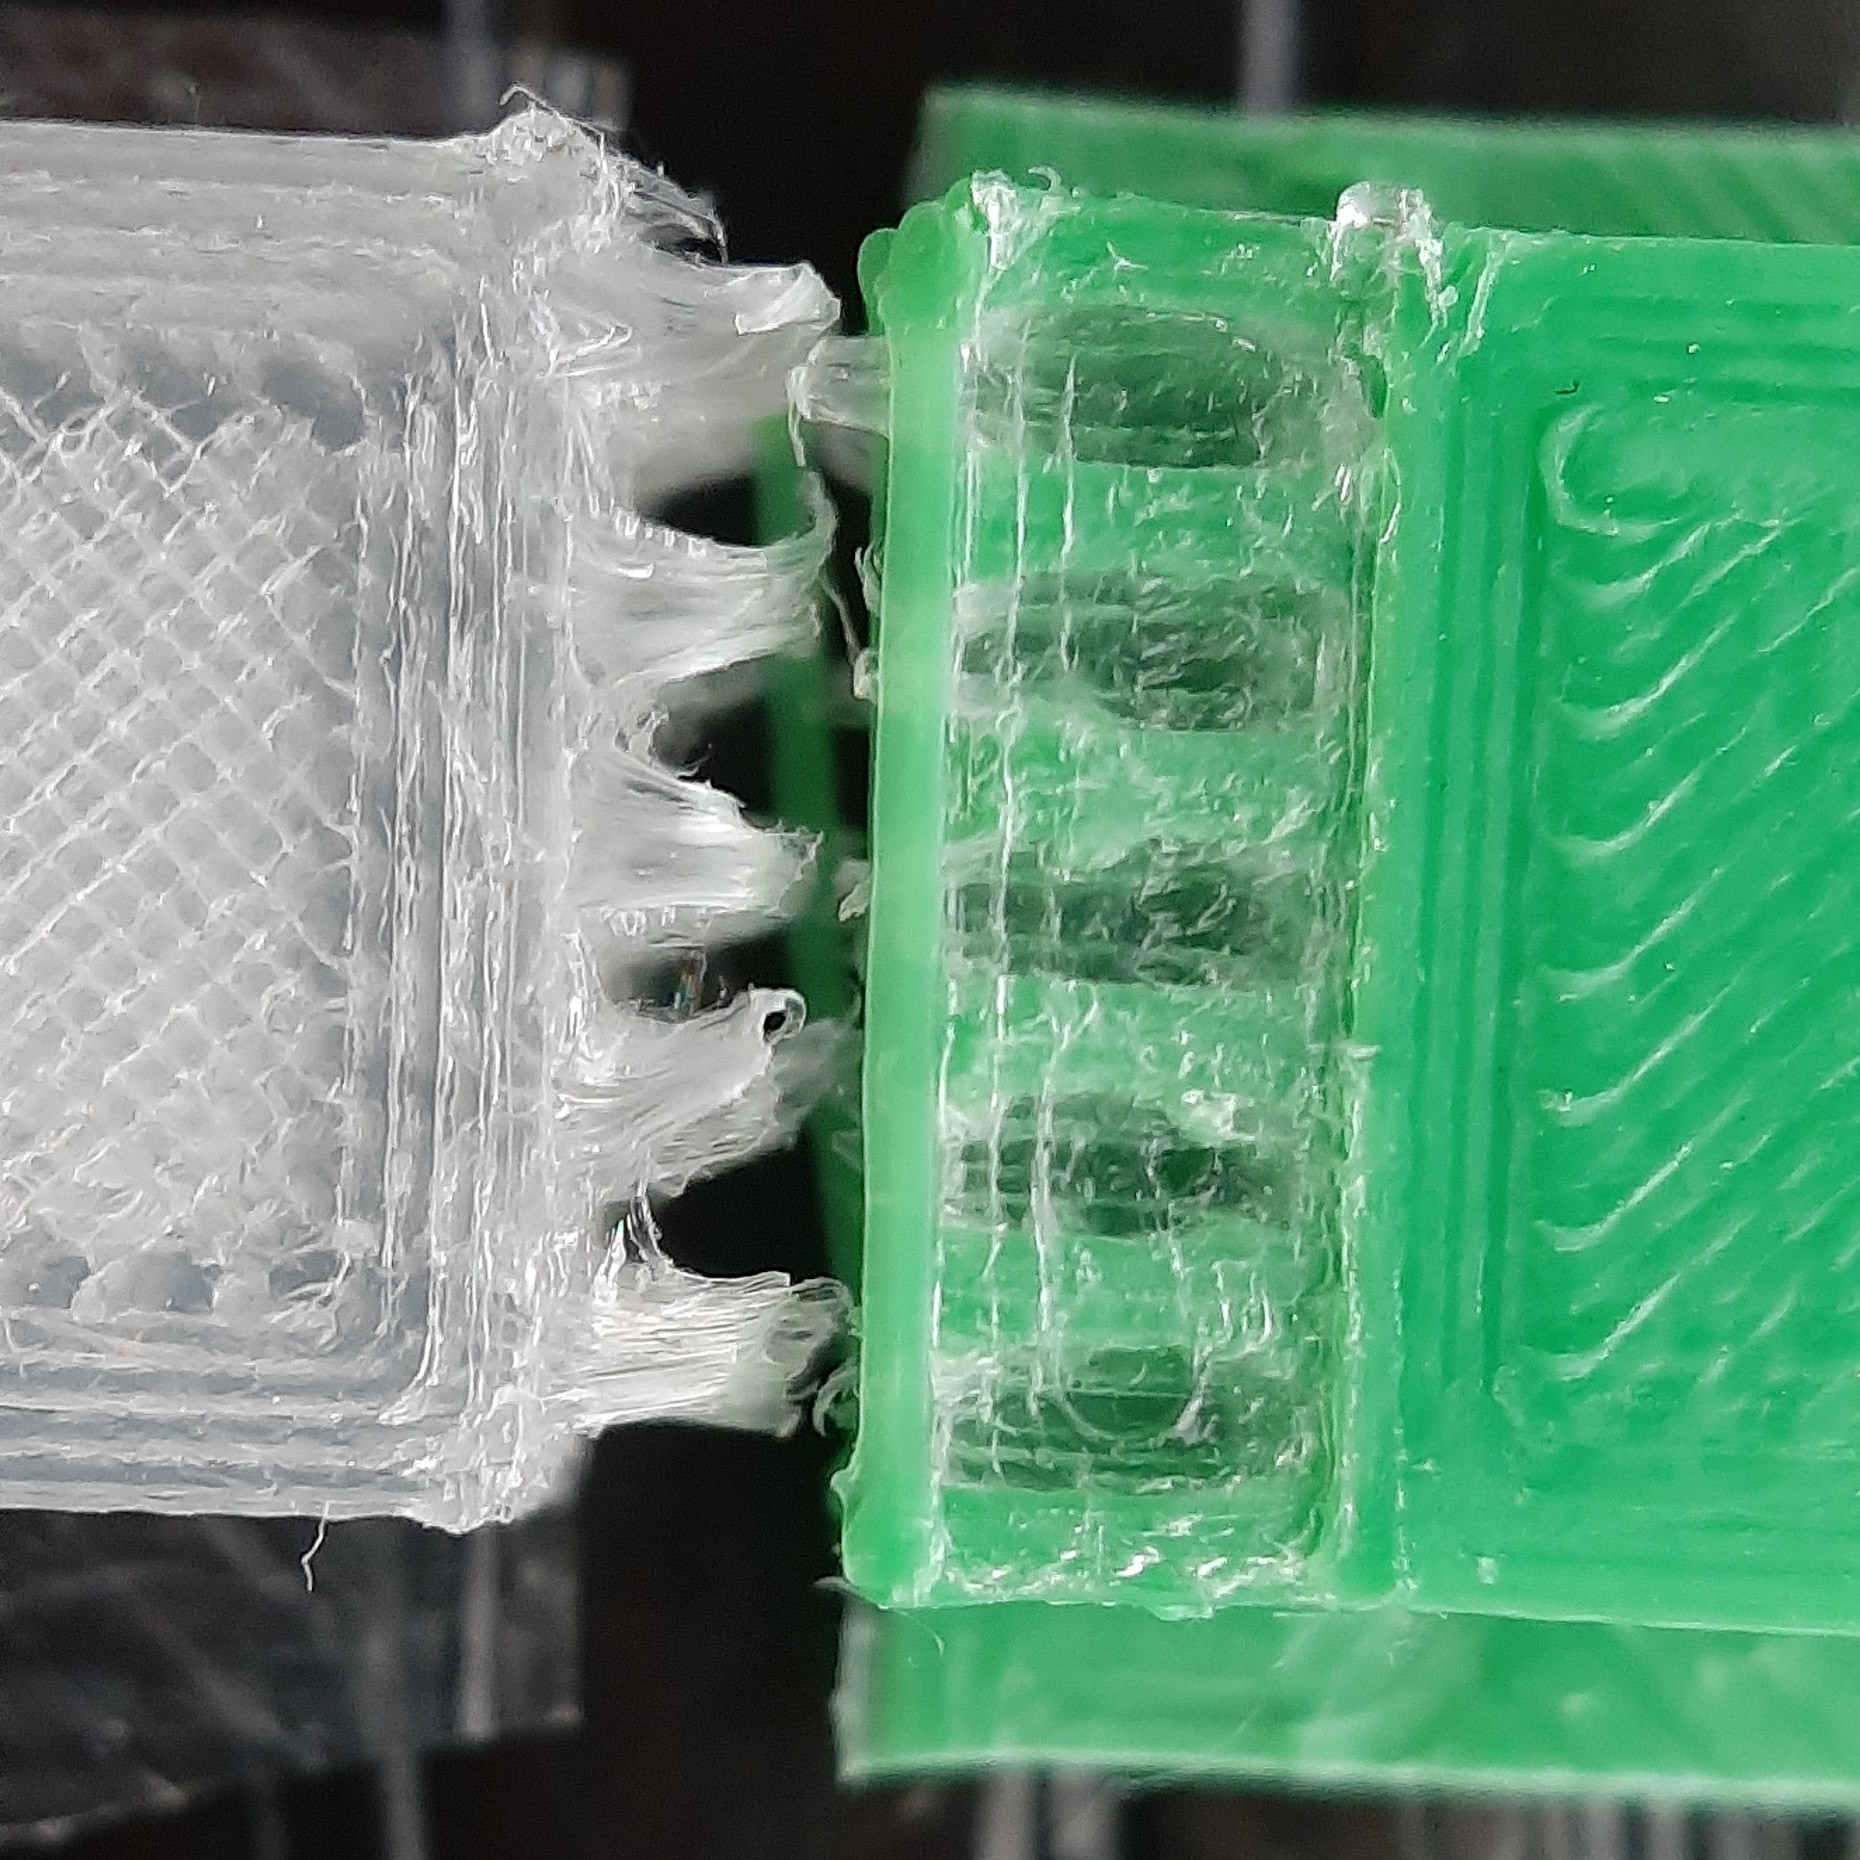
\includegraphics[width=\figwidth]{sources/testing/j4_cropped.jpg}
		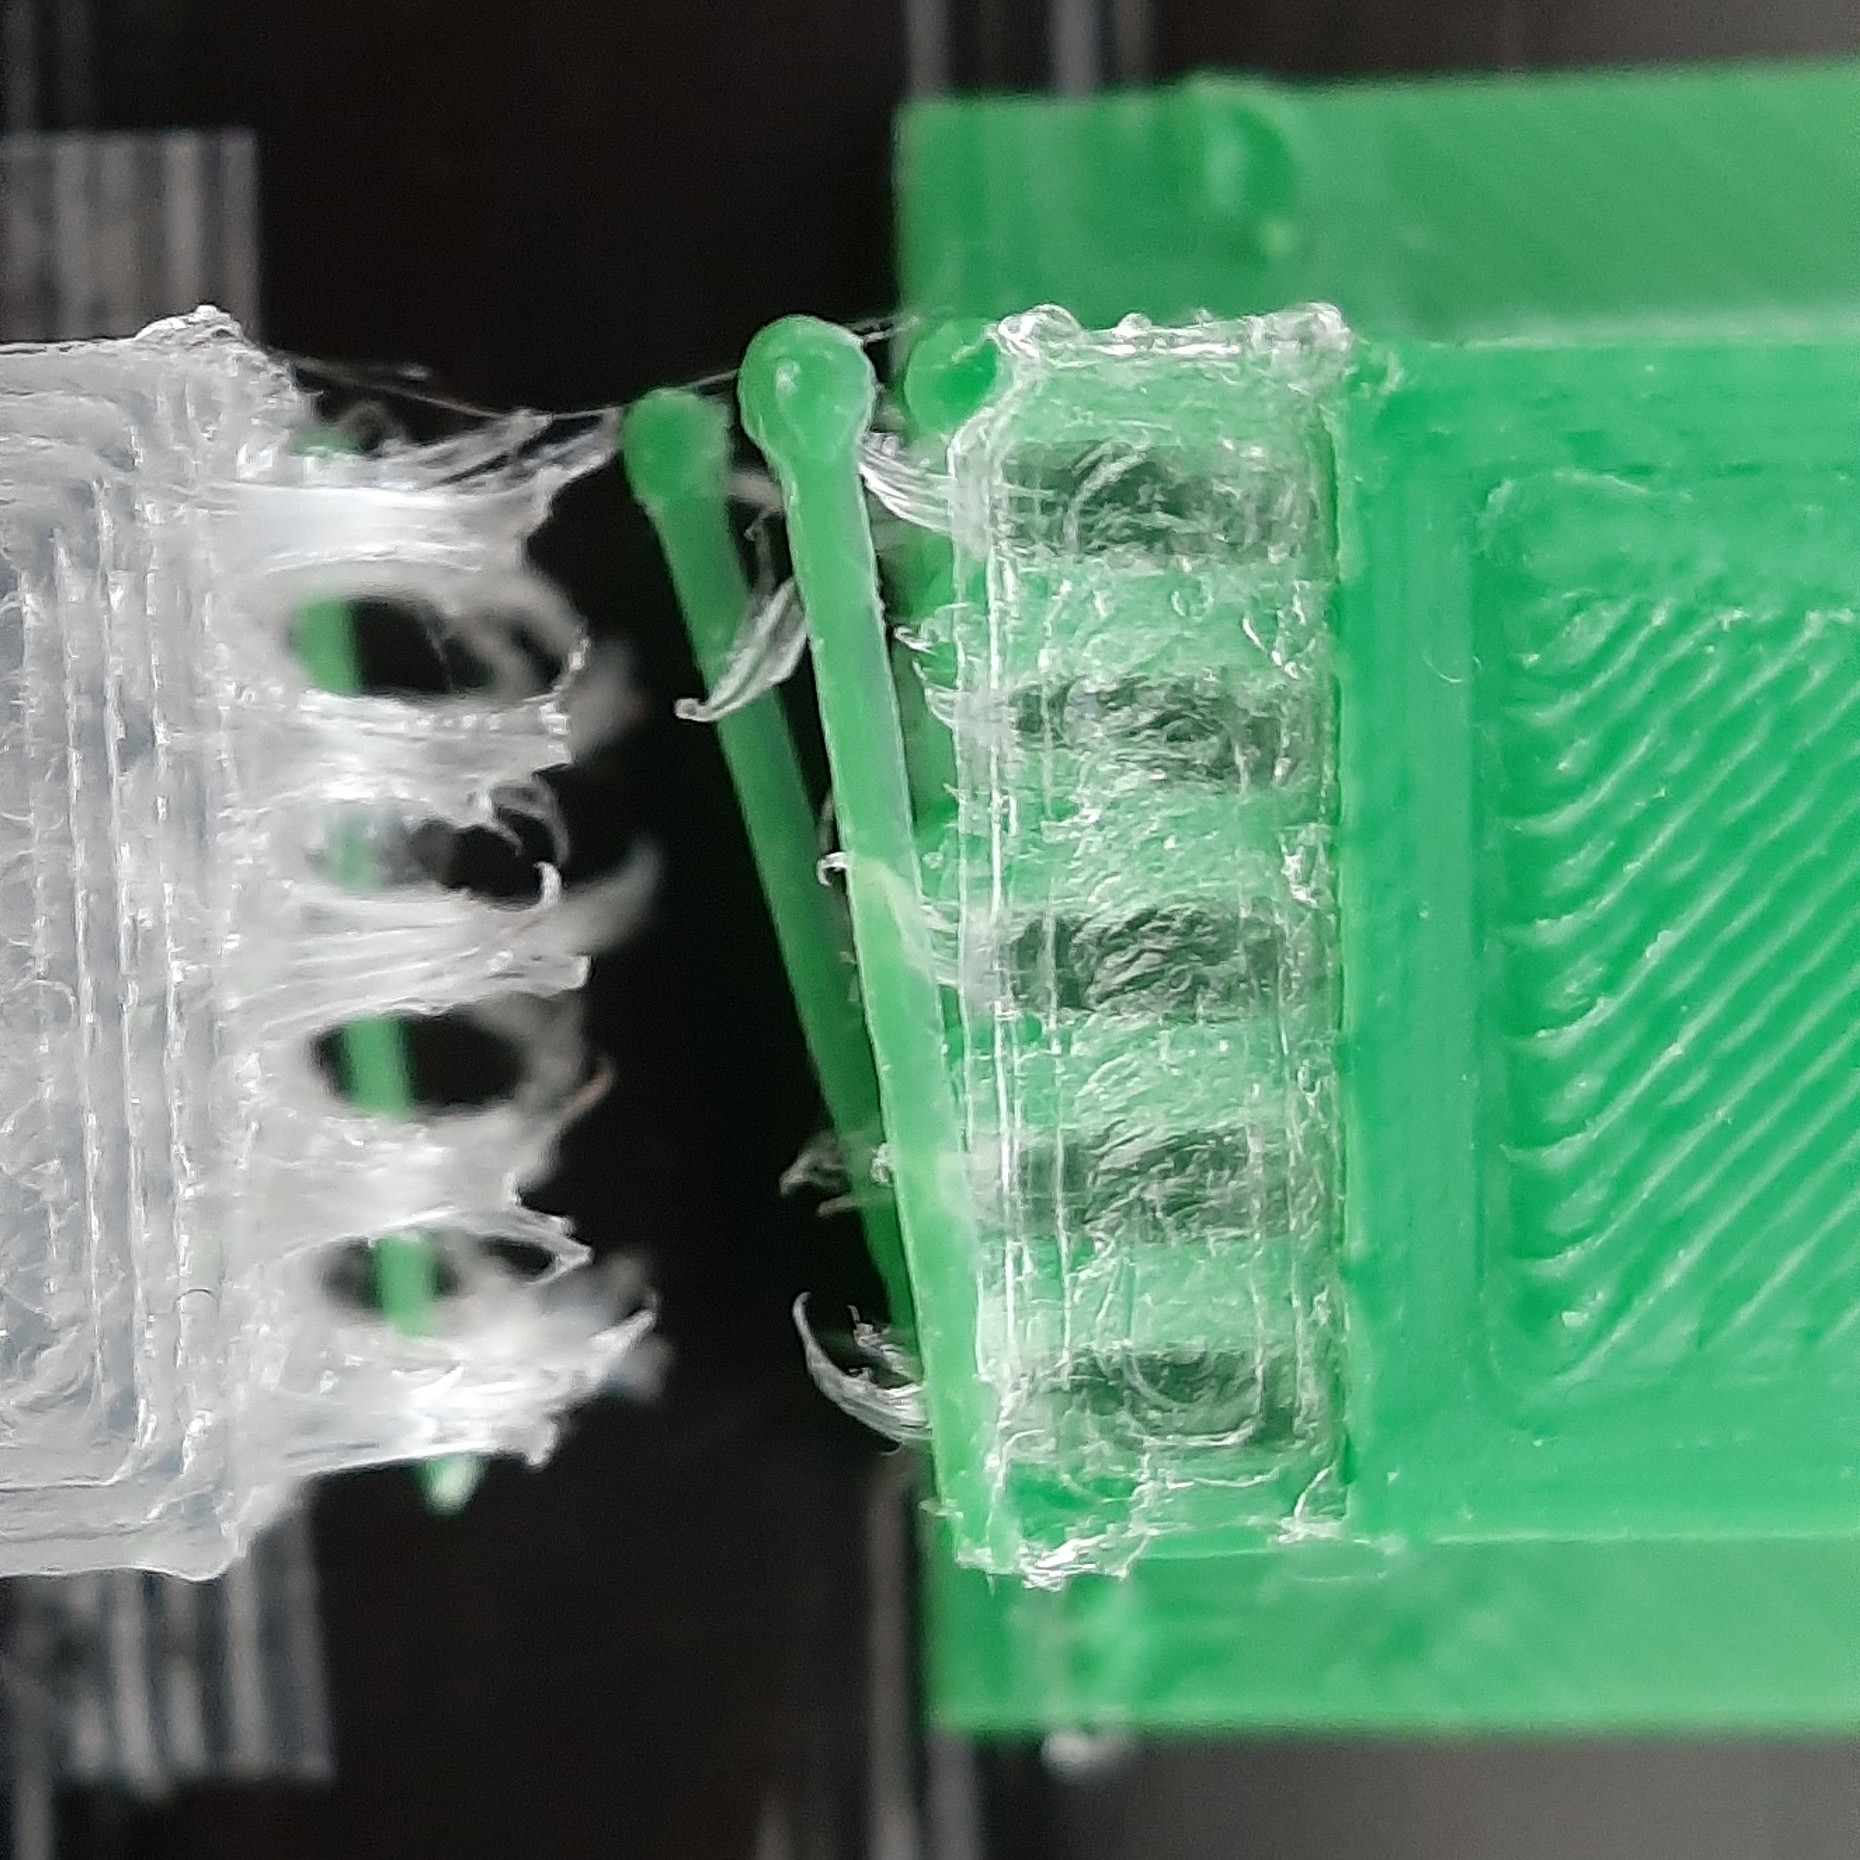
\includegraphics[width=\figwidth]{sources/testing/j5_cropped.jpg}
		\caption{Specimens after tensile test}
		\label{fig:failures}
	\end{subfigure}
	\caption{Tensile results for broken wb+: $\lmax=3.6, \wb=1.7, \va=0.3, \hf=0.5$}
\end{figure}


% table of best sample dimensions?



